
This part of the development process aims to realize a skeleton of the application and its main functionalities. The output of the process will be and application offering the possibility to visualize and partially handle a list of todos. It is composed by a single page: the HomePage. The HomePage is made of an AppBar and two tabs: the \textit{todos} tab and the \textit{stats} tab. \\
The \textit{todos} tab visualizes the list of todos. It is possible to filter todos using a DropdownButton widget situated in the top right corner, inside the AppBar. 
The available filter values are:
\begin{itemize}
    \item All (visualizes completed and pending todos)
    \item Completed (visualizes completed todo only)
    \item Not Completed (visualizes pending todos only)
\end{itemize}
The list of todos is visualized using a TodoView component widget. The elements contained in the TodoView component are called TodoItems. TodoItem widgets visualize the name, the description and the completion of a specific todo using two Text widgets and a Checkbox widget. It is possible to use the checkbox in order to mark a todo as completed or to mark it as pending depending on its current state. \\
The \textit{stats} tab visualizes the number of completed todos through a Text widget.
In the lower part, a TabSelector widget allow to switch from tabs.

\begin{figure}[H]
    \centering
    \subfloat[\textit{todos} tab runtime UI\label{fig:todos_tab_tree}]{
        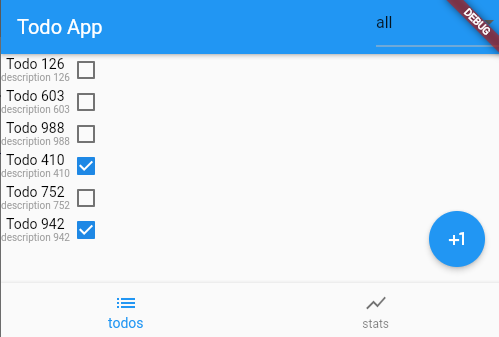
\includegraphics[scale=0.5]{Images/shot_runtime_todoapp_todos.png}
    }
    \quad
      \subfloat[\textit{stats} tab runtime UI.\label{fig:todos_tab_UI}]{
        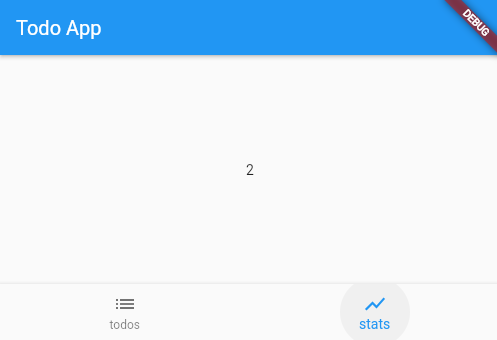
\includegraphics[scale=0.5]{Images/shot_runtime_todoapp_stats.png}
    }
    \caption{Shows the HomePage's UI }
    \label{fig:todos_tab}
\end{figure}